\documentclass{standalone}

\usepackage{pgfplots}

\begin{document}
	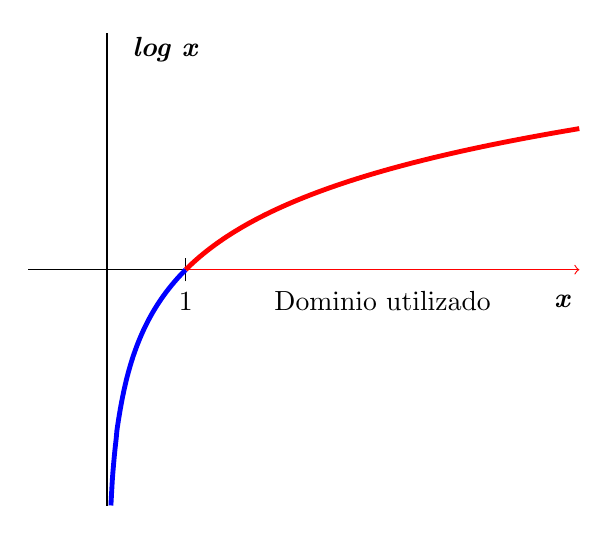
\begin{tikzpicture}
	\coordinate (LX) at (-1.00, 0.00); % left x
	\coordinate (RX1) at (1.00, 0.00); % right x 1
	\coordinate (RX2) at (6.00, 0.00); % right x 2
	\coordinate (BY) at (0.00, -3.00); % bottom y
	\coordinate (TY) at (0.00, 3.00); % top y

	\draw[-] (LX) -- (RX1);
	\draw[->, red] (RX1) -- (RX2);
	\node at (5.8,-0.4) {\textbf{\textit{x}}};
	\node at (3.5,-0.4) {Dominio utilizado};

	\draw[-] (BY) -- (TY);
	\node[right] at (0.2, 2.8) {\textbf{\textit{log x}}};

	\draw[-] (1,-0.15) -- (1,0.15);
	\node at (1, -0.4) {1};

	\draw[blue, line width=1.75pt, domain=0.05:1.00, samples=100] plot[smooth] (\x, {ln(\x)});
	\draw[red, line width=1.75pt, domain=1:6, samples=100] plot[smooth] (\x, {ln(\x)});
	\end{tikzpicture}
\end{document}
